\chapter{الكيمياء الحاسوبية: هارتري--فوك ونظرية دالية الكثافة}\label{ch:b3:computational-chemistry}

يُعتقد أن أيون هيدريد الهيليوم، \ce{HeH+}، هو أول جزيء
تكوّن حين برد الكون الفتي: ذرة هيليوم تمسك ببروتون. وقد
حُضّر في أنبوب تفريغ مخبري سنة 1925، لكن البحث عنه في الفضاء ظل
عقودًا دون جدوى، حتى رُصد خطه الدوراني في سديم
كوكبي سنة 2019. وكان طول رابطته وتردداته الاهتزازية
وأطوال موجات خطوطه معروفة منذ زمن طويل --- بفضل
الحساب. فبرنامج حاسوبي يحل، على وجه التقريب، \omterm{thm:b3:quantum-model-systems:schrodinger}{معادلة
شرودنغر} للإلكترونات يستطيع أن يتنبأ بشكل جزيء لم يضعه أحد في قارورة
وبطاقته وطيفه. يشرح هذا الفصل كيف تعمل هذه البرامج، من فصل النوى عن الإلكترونات
إلى نظرية هارتري--فوك \omterm{def:b3:computational-chemistry:dft}{ونظرية دالية الكثافة}، وفيمَ يمكن الوثوق بأعدادها
وفيمَ لا يمكن.

\begin{recall}
قدّم \cref{ch:b3:quantum-model-systems} \omterm{def:b3:quantum-model-systems:schrodinger}{مؤثر هاملتون} \omterm{thm:b3:quantum-model-systems:schrodinger}{ومعادلة شرودنغر}
وذرة الهيدروجين؛ وقدّم \cref{ch:b3:many-electron-atoms} \omterm{def:b3:many-electron-atoms:slater}{محدد سلاتر}
\omterm{def:b3:many-electron-atoms:exchange}{وتكامل التبادل}. وبنى مجلد السنة الثانية المدارات الجزيئية
تركيباتٍ خطية من المدارات الذرية (LCAO)، بتكاملات التداخل
وكولوم والرنين وبمحدد قرني، وحلّ
طريقة هوكل؛ واستعمل أيضًا أطياف الإلكترونات الضوئية لرؤية طاقات المدارات.
\end{recall}

\begin{omfigure}
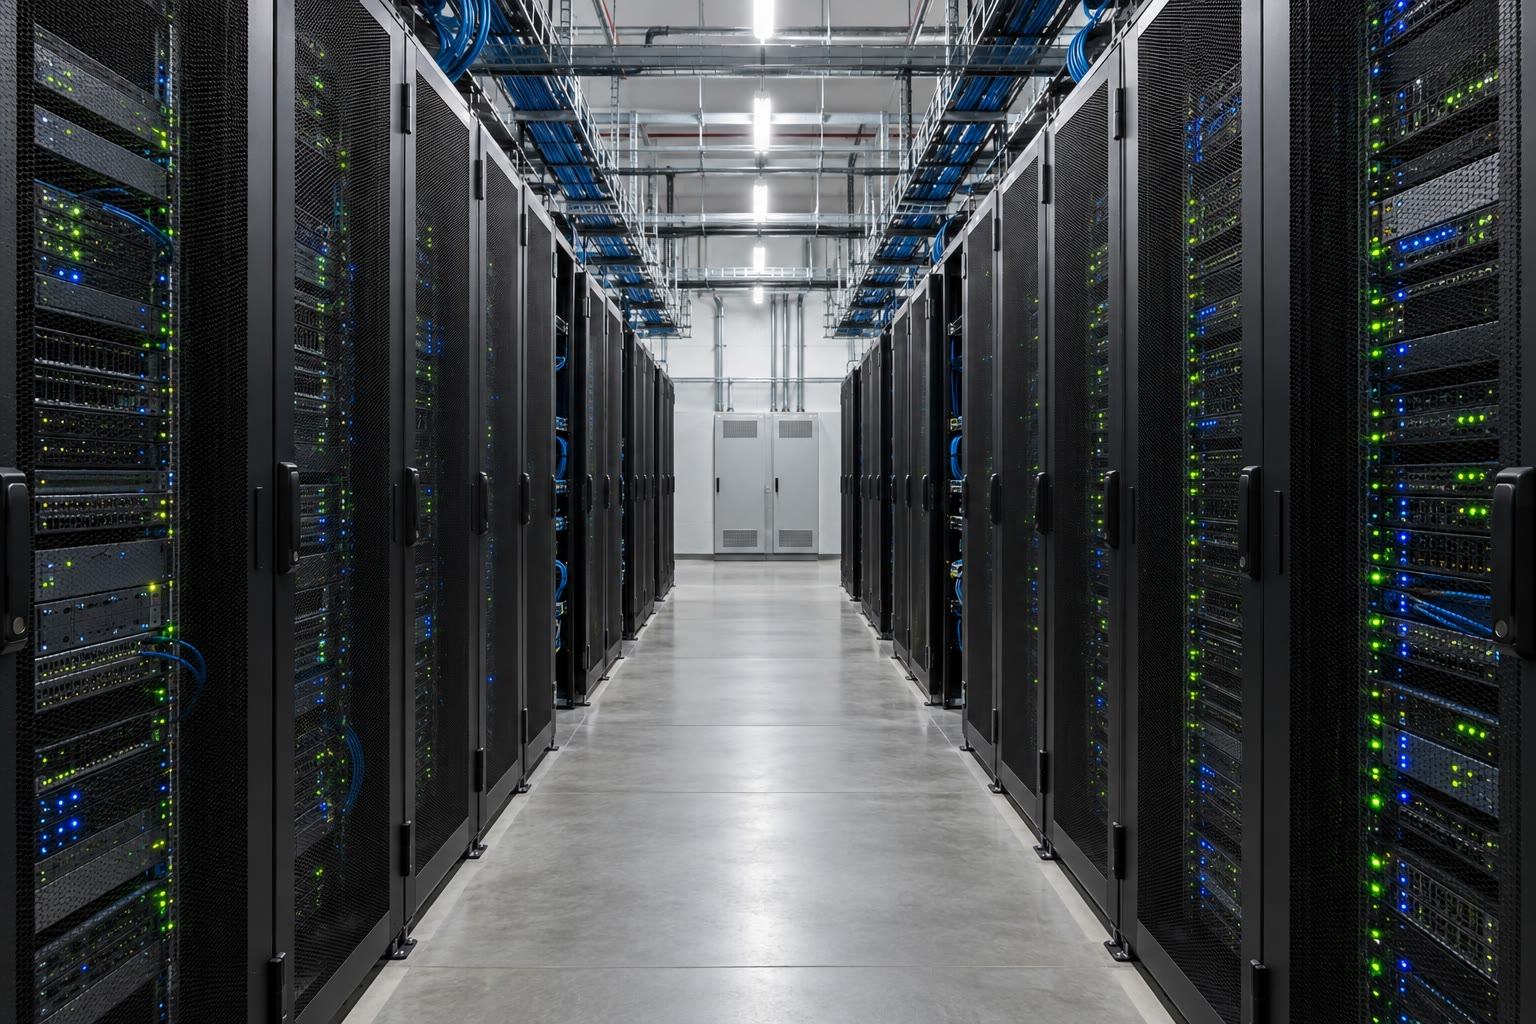
\includegraphics[width=0.6\linewidth]{images/book4/ai/b3-03-cluster.jpg}

{\small عنقود حوسبة: صفوف من الخوادم تجري عليها اليوم معظم حسابات
كيمياء الكم، وتستغرق غالبًا ساعات أو أيامًا لكل جزيء.}
\end{omfigure}

\section{تقريب بورن--أوبنهايمر وسطح الطاقة الكامنة}

يحتوي \omterm{def:b3:quantum-model-systems:schrodinger}{مؤثر هاملتون} للجزيء على الطاقات الحركية لنواه
وإلكتروناته وعلى كل تآثراتها الكولومية. والنوى أثقل من الإلكترونات بما لا يقل عن 1836
مرة: فهي تتحرك تحت القوى نفسها أبطأ بكثير، وتتكيف الإلكترونات
على الفور تقريبًا مع كل وضع
للنوى.

\begin{definition}[تقريب بورن--أوبنهايمر]\label{def:b3:computational-chemistry:born-oppenheimer}
في \emph{تقريب بورن--أوبنهايمر}\index{تقريب بورن--أوبنهايمر}،
تُحل \omterm{thm:b3:quantum-model-systems:schrodinger}{معادلة شرودنغر} الإلكترونية من أجل نوى
مثبّتة في المواضع $\mathbf R$،
\[
\hat H_{\mathrm{el}}\,\psi_{\mathrm{el}}(\mathbf r;\mathbf R) =
E_{\mathrm{el}}(\mathbf R)\,\psi_{\mathrm{el}}(\mathbf r;\mathbf R),
\]
ثم تتحرك النوى في الكمون $E_{\mathrm{el}}(\mathbf R) +
V_{\mathrm{nn}}(\mathbf R)$، أي الطاقة الإلكترونية مضافًا إليها تنافر
النوى.
\end{definition}

\begin{definition}[سطح الطاقة الكامنة، النقطة المستقرة، تحسين الهندسة]\label{def:b3:computational-chemistry:pes}
\emph{سطح الطاقة الكامنة}\index{سطح الطاقة الكامنة} (PES) للجزيء
هو الدالة $U(\mathbf R) = E_{\mathrm{el}}(\mathbf R) +
V_{\mathrm{nn}}(\mathbf R)$ لإحداثيات نواه. و\emph{النقطة
المستقرة}\index{نقطة مستقرة} نقطة تنعدم فيها كل المشتقات الأولى للدالة $U$؛
والقيمة الدنيا \emph{هندسة توازن}\index{هندسة توازن}.
والبحث عن إحداها انطلاقًا من بنية ابتدائية، باتباع
القوى $-\nabla U$، هو \emph{تحسين الهندسة}\index{تحسين الهندسة}.
\end{definition}

\omterm{def:b3:computational-chemistry:pes}{سطح الطاقة الكامنة} للجزيء الثنائي الذرة منحنى $U(R)$؛ وللجزيء الثلاثي الذرة
دالة في ثلاثة إحداثيات؛ ولجزيء من $N$ ذرة دالة في $3N - 6$ إحداثيًا. وكتلة
النوى لا تدخل في $\hat H_{\mathrm{el}}$: فالجزيئات \ce{H2} و\ce{HD} و\ce{D2} تشترك في
\omterm{def:b3:computational-chemistry:pes}{سطح الطاقة الكامنة} نفسه، وفي طول الرابطة \omterm{def:b3:quantum-model-systems:oscillator}{وثابت القوة} نفسيهما، ولا تختلف إلا في كيفية
حركة النوى عليه (\omterm{def:b3:quantum-model-systems:oscillator}{طاقة النقطة الصفرية}، \cref{ch:b3:quantum-model-systems}).

\begin{proposition}[الترددات من مصفوفة هيس]\label{prop:b3:computational-chemistry:hessian}
قرب قيمة دنيا، $U \approx U_0 + \frac12\sum_{ij}H_{ij}\,\delta q_i\,\delta q_j$، حيث
مصفوفة هيس $H_{ij} = \partial^2U/\partial q_i\partial q_j$. وفي الإحداثيات
المرجَّحة بالكتلة $\delta q_i\sqrt{m_i}$، تعطي القيم الذاتية $\lambda_k$ لمصفوفة
هيس المرجَّحة بالكتلة الترددات الزاوية التوافقية $\omega_k =
\sqrt{\lambda_k}$ للأنماط العادية. وعند القيمة الدنيا تكون كل القيم $\lambda_k$
موجبة (ست منها، أو خمس للجزيء الخطي، معدومة: الانسحابات
والدورانات)؛ وعند نقطة سرج من الرتبة الأولى تكون واحدة بالضبط سالبة.
\end{proposition}

\begin{proof}[برهان جزئي]
من أجل جزيء ثنائي الذرة، $U \approx U_0 + \frac12k(R - R_e)^2$ حيث $k = U''(R_e)$، 
ويعطي الهزاز في \cref{ch:b3:quantum-model-systems} العلاقة $\omega =
\sqrt{k/\mu}$. وفي الحالة العامة، تصير المعادلات الكلاسيكية $m_i\ddot q_i =
-\sum_jH_{ij}q_j$، بالإحداثيات المرجَّحة بالكتلة $x_i = \sqrt{m_i}q_i$،
$\ddot{\mathbf x} = -\tilde H\mathbf x$ مع المصفوفة المتناظرة $\tilde H_{ij} =
H_{ij}/\sqrt{m_im_j}$؛ وتهتز متجهاتها الذاتية مستقلةً بالتردد
$\sqrt{\lambda_k}$. والقيمة السالبة $\lambda_k$ تعطي ترددًا تخيليًا: ففي
ذلك الاتجاه تنخفض الطاقة، وهي قيمة عظمى. والأنماط العادية في
\cref{ch:b3:group-theory-applied} هي هذه المتجهات الذاتية.
\end{proof}

\begin{omfigure}
\begin{tikzpicture}[font=\small, scale=0.95]
  \fill[omDef!8] (0,0) ellipse (1.9 and 1.15);
  \foreach \s in {1.0,0.75,0.5,0.25}{\draw[omDef!70] (0,0) ellipse ({1.9*\s} and {1.15*\s});}
  \fill[omThm!8] (6,0.4) ellipse (1.6 and 1.0);
  \foreach \s in {1.0,0.75,0.5,0.25}{\draw[omThm!70] (6,0.4) ellipse ({1.6*\s} and {1.0*\s});}
  \draw[gray] (2.1,-0.15) .. controls (2.9,0.55) and (3.4,0.55) .. (4.3,0.35);
  \draw[gray] (2.2,0.9) .. controls (3.0,0.35) and (3.5,0.35) .. (4.1,1.2);
  \node[omsaddle] at (3.15,0.42) {};
  \draw[ompath] (0,0) .. controls (1.8,0.6) and (2.4,0.5) .. (3.15,0.42) .. controls (4.0,0.35) and (4.8,0.4) .. (6,0.4);
  \node[anchor=north] at (0,-1.25) {\shortstack{\foreignlanguage{arabic}{القيمة الدنيا \babelsublr{A} (المتفاعلات)}}};
  \node[anchor=north] at (6,-0.7) {\shortstack{\foreignlanguage{arabic}{القيمة الدنيا \babelsublr{B} (النواتج)}}};
  \node[anchor=south] at (3.15,1.25) {\foreignlanguage{arabic}{نقطة سرج}};
  \draw[->, gray] (3.15,1.25) -- (3.15,0.6);
  \fill (0,0) circle (1.2pt) (6,0.4) circle (1.2pt);
  \draw[->] (-2.3,-2.2) -- (8.2,-2.2) node[right] {$q_1$};
  \draw[->] (-2.3,-2.2) -- (-2.3,1.8) node[above] {$q_2$};
\end{tikzpicture}

{\small سطح طاقة كامنة منظورًا إليه من أعلى، في صورة خريطة خطوط تساوٍ على إحداثيين
نوويين (رسم تخطيطي). يصل بين قيمتين دنييين، مرورًا بنقطة سرج
(الصليب)، الطريقُ الأدنى طاقةً (متقطع): وهو طريق الطاقة الدنيا
الذي يدرسه \cref{ch:b3:rate-theories}.}
\end{omfigure}

\section{المبدأ التغايري}

لا يمكن حل \omterm{thm:b3:quantum-model-systems:schrodinger}{معادلة شرودنغر} الإلكترونية حلًا دقيقًا لأي
جزيء فيه أكثر من إلكترون واحد. وتُحاكم التقريبات بمبرهنة
واحدة.

\begin{theorem}[المبدأ التغايري]\label{thm:b3:computational-chemistry:variational}
من أجل أي دالة تجريبية قابلة للتنظيم $\phi$ تحقق الشروط
الحدية للمسألة،
\[
E[\phi] = \frac{\langle\phi|\hat H|\phi\rangle}{\langle\phi|\phi\rangle} \ge E_0,
\]
حيث $E_0$ أدنى \omterm{def:b3:quantum-model-systems:operator}{قيمة ذاتية} \omterm{def:b3:quantum-model-systems:operator}{للمؤثر} $\hat H$؛ ولا تتحقق المساواة إلا إذا كانت $\phi$
\omterm{def:b3:quantum-model-systems:operator}{دالة ذاتية} للحالة الأساسية. هذا هو \emph{المبدأ
التغايري}\index{مبدأ تغايري}.
\end{theorem}

\begin{proof}
لننشر $\phi = \sum_nc_n\psi_n$ على الدوال الذاتية المتعامدة المنظَّمة \omterm{def:b3:quantum-model-systems:operator}{للمؤثر} $\hat H$
(\cref{thm:b3:quantum-model-systems:hermitian-real}). عندئذ $\langle\phi|\hat
H|\phi\rangle = \sum_n|c_n|^2E_n \ge E_0\sum_n|c_n|^2 = E_0\langle\phi|\phi\rangle$،
لأن كل $E_n \ge E_0$؛ والمساواة تقتضي $c_n = 0$ كلما كان $E_n > E_0$.
\end{proof}

كلما انخفضت طاقة الدالة التجريبية كانت أفضل؛ وكل وسيط قابل
للضبط يُثبَّت بجعل $E$ أصغر ما يمكن.

\begin{proposition}[الهيليوم بشحنة محجوبة]\label{prop:b3:computational-chemistry:helium-zeta}
من أجل الهيليوم، تعطي الدالة التجريبية $\phi = \eu^{-\zeta(r_1 + r_2)}$ (بالوحدات الذرية:
الأطوال بوحدة $a_0$، والطاقات بوحدة $E_h$) العلاقة $E(\zeta) = \zeta^2 - \frac{27}{8}\zeta$،
وهي أصغر ما يمكن من أجل $\zeta = \frac{27}{16}$، حيث $E = -(\frac{27}{16})^2 E_h =
\qty{-2.8477}{\hartree}$.
\end{proposition}

\begin{proof}
من أجل إلكترون واحد في $\eu^{-\zeta r}$، $\langle T\rangle = \zeta^2/2$ 
و$\langle 1/r\rangle = \zeta$؛ وتنافر إلكترونين في الدالة $1s$ نفسها
هو $\frac58\zeta$ (تكامل معروف، نقبله دون برهان). ومنه $E = 2\cdot\frac12
\zeta^2 - 2\cdot2\zeta + \frac58\zeta = \zeta^2 - \frac{27}{8}\zeta$، و$\dd E/\dd
\zeta = 0$ تعطي $\zeta = 27/16 = 1.6875$.
\end{proof}

\begin{example}[ما مدى جودته؟]\label{ex:b3:computational-chemistry:helium}
% ledger: ie:He, ie4:He2, const:Eh, const:eV
الطاقة الكلية للهيليوم هي سالب مجموع طاقتي تأينه،
$-(24.5874 + 54.4178)\,\unit{eV} = \qty{-2.9034}{\hartree}$. والدالة ذات
الوسيط الواحد أعلى بمقدار \qty{0.056}{\hartree} (\qty{1.5}{eV}): فكل إلكترون يرى
نواة محجوبة إلى $Z_{\mathrm{eff}} = 1.69$ بفعل الآخر، كما توحي
قواعد سلاتر، لكن الإلكترونين يتفادى أحدهما الآخر أيضًا على نحو لا يستطيع أي جداء
لدالتين أن يصفه.
\end{example}

\begin{proposition}[التغاير الخطي]\label{prop:b3:computational-chemistry:linear-variation}
من أجل دالة تجريبية $\phi = \sum_{i=1}^n c_i\chi_i$ مبنية على $n$ دالة ثابتة،
مع $H_{ij} = \langle\chi_i|\hat H|\chi_j\rangle$ و$S_{ij} = \langle\chi_i|\chi_j
\rangle$، تكون القيم المستقرة للطاقة $E$ جذور $\det(H - ES) = 0$، 
وأصغر جذر حد أعلى للطاقة $E_0$.
\end{proposition}

\begin{proof}
$E\sum_{ij}c_ic_jS_{ij} = \sum_{ij}c_ic_jH_{ij}$ (معاملات حقيقية). لنشتق
بالنسبة إلى $c_k$ ولنضع $\partial E/\partial c_k = 0$: $\sum_j(H_{kj} -
ES_{kj})c_j = 0$ من أجل كل $k$. ويقتضي وجود حل غير معدوم انعدام
المحدد. وأصغر جذر هو $E[\phi]$ من أجل متجهته الذاتية، ومنه $\ge E_0$.
\end{proof}

طريقة هوكل في مجلد السنة الثانية هي هذه القضية مع مدارات $p$
وعناصر $H_{ij}$ تجريبية. وكل طريقة فيما يلي هي الفكرة نفسها مع
دوال أفضل وعناصر مصفوفة أفضل.

\section{مجموعات الأساس}

\begin{definition}[مجموعة الأساس، الأساس الأدنى، المدارات من نمط سلاتر ونمط غاوس]\label{def:b3:computational-chemistry:basis}
\emph{مجموعة الأساس}\index{مجموعة أساس} هي مجموعة الدوال الثابتة $\chi_i$،
المتمركزة على الذرات، التي تُبنى منها المدارات الجزيئية. 
و\emph{مجموعة الأساس الدنيا}\index{مجموعة أساس دنيا} فيها دالة واحدة لكل
مدار ذري مشغول (دالة $1s$ واحدة للهيدروجين، وخمس للكربون). و\emph{المدار من نمط
سلاتر}\index{مدار من نمط سلاتر} (STO) شكله الشعاعي
$r^{n-1}\eu^{-\zeta r}$؛ و\emph{المدار من نمط غاوس}\index{مدار من نمط غاوس}
(GTO) شكله $\eu^{-\alpha r^2}$ مضروبًا في كثير حدود في $x$ و$y$
و$z$. و\emph{الدالة الغاوسية المقلَّصة}\index{دالة غاوسية مقلصة}
تركيب ثابت $\sum_kd_k\,\eu^{-\alpha_kr^2}$ لدوال غاوسية أولية.
\end{definition}

لدوال سلاتر الشكل الصحيح (رأس مدبّب عند النواة، وذيل
أسي) لكن تكاملاتها الثنائية الإلكترون على عدة مراكز
مكلفة جدًا؛ أما الدوال الغاوسية فشكلها خاطئ، لكن جداء دالتين
غاوسيتين على مركزين مختلفين دالة غاوسية على نقطة بينهما، فيؤول
كل تكامل إلى علاقة مغلقة. والتقليص يأخذ أفضل ما في
الاثنتين: ففي الأساس STO-3G، تُستبدل بكل دالة سلاتر مجموعٌ ثابت من
ثلاث دوال غاوسية مضبوطة عليها.

\begin{example}[دالة الهيدروجين في الأساس STO-3G]\label{ex:b3:computational-chemistry:sto3g}
% ledger: bse:H.sto3g.a1, bse:H.sto3g.a2, bse:H.sto3g.a3, bse:sto3g.c1, bse:sto3g.c2, bse:sto3g.c3
دالة $1s$ للهيدروجين في الأساس STO-3G هي $0.15433\,g(3.42525) + 0.53533\,
g(0.62391) + 0.44463\,g(0.16886)$، حيث $g(\alpha)$ الدالة الغاوسية المنظَّمة
$(2\alpha/\pi)^{3/4}\eu^{-\alpha r^2}$ (الأسس بوحدة $a_0^{-2}$). وهي تحاكي
دالة سلاتر أسّها $\zeta = 1.24$ --- أي ذرة هيدروجين مضغوطة
قليلًا، كما هي في الجزيئات. وتداخلها مع دالة $1s$ الدقيقة
ذات الأس نفسه $0.9998$؛ ولا يفوتها إلا الرأس المدبّب عند النواة والذيل
البعيد (الشكل أدناه).
\end{example}

\begin{definition}[دوال التكافؤ المجزأ والاستقطاب والدوال المنتشرة]\label{def:b3:computational-chemistry:split-valence}
تصف \emph{مجموعة الأساس مجزأة التكافؤ}\index{مجموعة أساس مجزأة التكافؤ} كل
مدار تكافؤ بدالتين (أو أكثر) مختلفتي الحجم، كي يستطيع
المدار أن يتمدد أو يتقلص في الجزيء. و\emph{دالة
الاستقطاب}\index{دالة استقطاب} لها $l$ أعلى من المدارات
المشغولة ($p$ على H، و$d$ على C) وتسمح للكثافة بالانزياح خارج الذرة؛ 
و\emph{الدالة المنتشرة}\index{دالة منتشرة} لها أس صغير 
وتصف الأنيونات والتآثرات الضعيفة بعيدًا عن النوى.
\end{definition}

اسم مثل 6-31G(d) يقول: ست دوال أولية لكل دالة داخلية، 
وتكافؤ مجزأ إلى تقليص من ثلاث ودالة أولية مفردة، ودوال
استقطاب $d$ على الذرات الثقيلة. وتتقارب النتائج نحو
\emph{نهاية \omterm{def:b3:computational-chemistry:basis}{مجموعة الأساس}} كلما كبر الأساس؛ فالحساب لا يكون أفضل من
أساسه.

\begin{omfigure}
\begin{tikzpicture}
\begin{axis}[width=0.46\linewidth, height=5.4cm, xmin=0, xmax=5, ymin=0,
  ymax=0.6, axis lines=left, xlabel={\babelsublr{$r$ / $a_0$}}, ylabel={$\phi(r)$},
  legend cell align=left, legend style={font=\small, draw=none},
  tick label style={font=\small}, label style={font=\small},
  title={\small \foreignlanguage{arabic}{\babelsublr{STO-3G} مقابل $\eu^{-r}$ \babelsublr{($\zeta = 1$)}}}]
\addplot[black, thick] table[x=r, y=slater] {figdata/out/bachelor-3-minimal-basis-hf-sto.dat};
\addlegendentry{\foreignlanguage{arabic}{سلاتر}}
\addplot[omDef, thick, dashed] table[x=r, y=g3] {figdata/out/bachelor-3-minimal-basis-hf-sto.dat};
\addlegendentry{STO-3G}
\addplot[omThm, thick, dotted] table[x=r, y=g1] {figdata/out/bachelor-3-minimal-basis-hf-sto.dat};
\addlegendentry{\foreignlanguage{arabic}{دالة غاوسية واحدة}}
\end{axis}
\end{tikzpicture}\hfill
\begin{tikzpicture}
\begin{axis}[width=0.46\linewidth, height=5.4cm, xmin=0.5, xmax=8.5,
  ymin=-2.86, ymax=-2.78, axis lines=left, xlabel={\foreignlanguage{arabic}{دورة \babelsublr{SCF}}},
  ylabel={\babelsublr{$E$ / $E_h$}}, ytick={-2.85,-2.83,-2.81,-2.79},
  yticklabel style={/pgf/number format/fixed, /pgf/number format/precision=2},
  tick label style={font=\small}, label style={font=\small},
  title={\small \foreignlanguage{arabic}{دورات \babelsublr{SCF} للأيون \ce{HeH+}}}]
\addplot[omDef, thick, mark=*] table[x=it, y=E] {figdata/out/bachelor-3-minimal-basis-hf-heh-scf.dat};
\addplot[gray, dashed, domain=0.5:8.5] {-2.84184};
\end{axis}
\end{tikzpicture}

{\small يسارًا: يعيد التقليص STO-3G (متقطع) دالة سلاتر $1s$
بدقة إلا عند النواة؛ أما الدالة الغاوسية الواحدة (منقّط) فلا.
يمينًا: طاقة \ce{HeH+} عند \qty{1.4632}{\bohr} خلال تكرارات
\omterm{def:b3:computational-chemistry:hartree-fock}{المجال المتسق ذاتيًا} (STO-3G)؛ وهي تتقارب من أعلى نحو
\qty{-2.8418}{\hartree} في بضع دورات، وكل تكرار يخضع \omterm{thm:b3:computational-chemistry:variational}{للمبدأ
التغايري}.}
\end{omfigure}

\section{نظرية هارتري--فوك}

أبسط \omterm{def:b3:many-electron-atoms:indistinguishable}{دالة موجية ضد متناظرة} لعدد $N$ من الإلكترونات \omterm{def:b3:many-electron-atoms:slater}{محدد سلاتر}
واحد. ونظرية هارتري--فوك تجد أفضلها.

\begin{definition}[طريقة هارتري--فوك، مؤثر فوك، المجال المتسق ذاتيًا]\label{def:b3:computational-chemistry:hartree-fock}
تقرّب \emph{طريقة هارتري--فوك}\index{طريقة هارتري--فوك}
الحالة الأساسية \omterm{def:b3:many-electron-atoms:slater}{بمحدد سلاتر} الوحيد ذي الطاقة الدنيا. ومداراته
دوال ذاتية \emph{لمؤثر فوك}\index{مؤثر فوك}
\[
\hat f(1) = \hat h(1) + \sum_b\big[2\hat J_b(1) - \hat K_b(1)\big],
\]
في حالة الطبقات المغلقة: $\hat h$ هو الطاقة الحركية لإلكترون واحد وتجاذبه مع
النوى، و$\hat J_b$ التنافر مع سحابة شحنة
المدار $b$، و$\hat K_b$ \omterm{def:b3:quantum-model-systems:operator}{مؤثر} التبادل، الذي قيمه المتوقعة هي
تكاملات التبادل في \cref{ch:b3:many-electron-atoms}. وبما أن $\hat f$
يتعلق بالمدارات التي يحددها، تُحل المعادلات
بالتكرار حتى تكف المدارات عن التغير: وهذا \emph{المجال المتسق
ذاتيًا}\index{مجال متسق ذاتيًا} (SCF).
\end{definition}

\begin{theorem}[معادلات روثان--هول]\label{thm:b3:computational-chemistry:roothaan}
بكتابة كل مدار في أساس، $\phi_a = \sum_\mu C_{\mu a}\chi_\mu$، تصير
معادلات هارتري--فوك للطبقات المغلقة مسألة القيم الذاتية المصفوفية
\[
\mathbf F\mathbf C = \mathbf S\mathbf C\boldsymbol\varepsilon, \qquad F_{\mu\nu} =
h_{\mu\nu} + \sum_{\lambda\sigma}P_{\lambda\sigma}\big[(\mu\nu|\sigma\lambda) -
\tfrac12(\mu\lambda|\sigma\nu)\big],
\]
مع مصفوفة الكثافة $P_{\lambda\sigma} = 2\sum_a^{\mathrm{occ}}C_{\lambda a}C_{\sigma
a}$ والتكاملات الثنائية الإلكترون $(\mu\nu|\lambda\sigma) = \iint\chi_\mu(1)\chi_\nu(1)
r_{12}^{-1}\chi_\lambda(2)\chi_\sigma(2)$ (وحدات ذرية).
\end{theorem}

\begin{proof}[برهان جزئي]
طاقة المحدد هي $E = \sum_{\mu\nu}P_{\mu\nu}h_{\mu\nu} + \frac12
\sum P_{\mu\nu}P_{\lambda\sigma}[(\mu\nu|\sigma\lambda) - \frac12(\mu\lambda|\sigma\nu)]$، وهي
دالة تربيعية في المعاملات. لنجعلها أصغر ما يمكن تحت القيود
التي تُبقي المدارات متعامدة منظَّمة، $\mathbf C^{\mathsf T}\mathbf S\mathbf C = \mathbf 1$،
بمضروب لاغرانج لكل قيد: فتكون شروط
الاستقرار $\mathbf F\mathbf C = \mathbf S\mathbf C\boldsymbol\varepsilon$، 
وتشكّل المضاريب مصفوفة يمكن جعلها قطرية بتدوير
المدارات المشغولة فيما بينها. ونقبل الجبر دون برهان.
\end{proof}

\begin{method}[إجراء المجال المتسق ذاتيًا]\label{met:b3:computational-chemistry:scf}
\begin{enumerate}
  \item احسب التكاملات $S_{\mu\nu}$ و$h_{\mu\nu}$ و$(\mu\nu|\lambda\sigma)$ مرة واحدة.
  \item خمّن مصفوفة الكثافة (مثلًا من المتجهات الذاتية
        للمصفوفة $\mathbf h$ وحدها، وهو تخمين «القلب»).
  \item ابنِ $\mathbf F$ من $\mathbf P$؛ وحُلّ $\mathbf F\mathbf C = \mathbf S\mathbf C
        \boldsymbol\varepsilon$ (عامِد بالمصفوفة $\mathbf S^{-1/2}$، ثم اجعلها قطرية).
  \item املأ المدارات الأدنى، بإلكترونين لكل منها؛ وكوّن $\mathbf P$ الجديدة
        والطاقة.
  \item كرّر انطلاقًا من الخطوة 3 حتى يصبح تغيّر الطاقة و$\mathbf P$ أقل من
        عتبة معينة.
\end{enumerate}
\end{method}

\begin{omfigure}
\begin{tikzpicture}[font=\small, node distance=4mm,
  box/.style={draw=black!60, rounded corners=2pt, fill=omDef!6, align=center,
  text width=4.4cm, inner sep=4pt}]
  \node[box] (a) {\foreignlanguage{arabic}{التكاملات $S$ و$h$ و$(\mu\nu|\lambda\sigma)$}};
  \node[box, below=of a] (b) {\foreignlanguage{arabic}{خمّن $\mathbf P$}};
  \node[box, below=of b] (c) {\foreignlanguage{arabic}{ابنِ $\mathbf F(\mathbf P)$}};
  \node[box, below=of c] (d) {\foreignlanguage{arabic}{حُلّ $\mathbf F\mathbf C = \mathbf S\mathbf C\boldsymbol\varepsilon$}};
  \node[box, below=of d] (e) {\foreignlanguage{arabic}{$\mathbf P$ الجديدة، والطاقة $E$}};
  \node[diamond, aspect=2.4, draw=black!60, fill=omThm!6, below=of e, inner sep=1pt] (f) {\foreignlanguage{arabic}{تقارب؟}};
  \node[box, below=of f, fill=omProp!8] (g) {\foreignlanguage{arabic}{المدارات، $\varepsilon$، $E$}};
  \draw[->] (a) -- (b); \draw[->] (b) -- (c); \draw[->] (c) -- (d);
  \draw[->] (d) -- (e); \draw[->] (e) -- (f);
  \draw[->] (f) -- node[left] {\foreignlanguage{arabic}{نعم}} (g);
  \draw[->] (f.east) -- ++(1.6,0) |- node[pos=0.25, right] {\foreignlanguage{arabic}{لا}} (c.east);
\end{tikzpicture}

{\small حلقة \omterm{def:b3:computational-chemistry:hartree-fock}{المجال المتسق ذاتيًا} في حساب هارتري--فوك.}
\end{omfigure}

\begin{example}[\ce{H2} في الأساس الأدنى]\label{ex:b3:computational-chemistry:h2}
% ledger: re:H2, janaf:H.dfH0, diat:H2.we, diat:H2.wexe
بدالة STO-3G واحدة لكل ذرة، يتحدد المدار الرابط بالتناظر،
$\sigma_g \propto \chi_A + \chi_B$، ولا يحتاج \omterm{def:b3:computational-chemistry:hartree-fock}{المجال المتسق ذاتيًا} إلا إلى خطوة واحدة. وعند $R =
\qty{1.4}{\bohr}$ يكون التداخل $S_{AB} = 0.6593$ والطاقة
\qty{-1.1167}{\hartree}؛ وتقع القيمة الدنيا عند \qty{1.346}{\bohr} (\qty{71.2}{pm}،
مقابل \qty{74.1}{pm} المقيسة) و\qty{-1.1175}{\hartree}. ويقارن الشكل أدناه
المنحنى بالمنحنى الحقيقي، المبني من معطيات طيفية
مقيسة ومن طاقة التفكك (منحنى مورس، \cref{ch:b3:rovibrational-spectroscopy}).
\end{example}

\begin{omfigure}
\begin{tikzpicture}
\begin{axis}[width=0.7\linewidth, height=6cm, xmin=0.8, xmax=10, ymin=-1.2,
  ymax=-0.45, axis lines=left, xlabel={\babelsublr{$R$ / $a_0$}}, ylabel={\babelsublr{$E$ / $E_h$}},
  legend cell align=left, legend style={font=\small, at={(0.04,0.98)}, anchor=north west, draw=none},
  tick label style={font=\small}, label style={font=\small}]
\addplot[omDef, thick] table[x=R, y=rhf] {figdata/out/bachelor-3-minimal-basis-hf-h2.dat};
\addlegendentry{RHF/STO-3G}
\addplot[black, thick, dashed] table[x=R, y=morse] {figdata/out/bachelor-3-minimal-basis-hf-h2.dat};
\addlegendentry{\foreignlanguage{arabic}{مقيس، بصيغة مورس}}
\addplot[gray, dotted, domain=0.8:10] {-1.0};
\addplot[omThm, dotted, domain=0.8:10] {-0.93316};
\node[font=\scriptsize, anchor=north] at (axis cs:8,-1.005) {\foreignlanguage{arabic}{ذرتا \babelsublr{H} دقيقتان}};
\node[font=\scriptsize, anchor=south, omThm] at (axis cs:8,-0.930) {\foreignlanguage{arabic}{ذرتا \babelsublr{H} في الأساس \babelsublr{STO-3G}}};
\end{axis}
\end{tikzpicture}

{\small طاقة \ce{H2} بدلالة المسافة بين النواتين: \omterm{def:b3:computational-chemistry:hartree-fock}{طريقة
هارتري--فوك} المقيَّدة في الأساس STO-3G (متصل) والمنحنى الحقيقي (متقطع، بصيغة
مورس المبنية من $D_0$ و$\omega_e$ و$\omega_ex_e$ و$r_e$ المقيسة). قرب
القيمة الدنيا تكون RHF جيدة؛ أما عند $R$ الكبيرة فترتفع كثيرًا فوق ذرتي هيدروجين.}
\end{omfigure}

\begin{proposition}[لماذا تخفق طريقة هارتري--فوك المقيَّدة عند التفكك]\label{prop:b3:computational-chemistry:rhf-dissociation}
في الأساس الأدنى، الدالة الموجية RHF للجزيء \ce{H2} هي، بإهمال
عامل التنظيم، $\sigma_g(1)\sigma_g(2) \propto \chi_A(1)\chi_B(2) + \chi_B(1)\chi_A(2)
+ \chi_A(1)\chi_A(2) + \chi_B(1)\chi_B(2)$: فهي عند أي مسافة نصف تساهمية ونصف
أيونية (\ce{H+ H-}). وعند $R$ الكبيرة تؤول طاقتها إلى متوسط طاقة ذرتين
متعادلتين وطاقة زوج أيوني، لا إلى طاقة ذرتين.
\end{proposition}

\begin{proof}
لننشر $(\chi_A + \chi_B)(1)(\chi_A + \chi_B)(2)$: يضع الحدان المتقاطعان
إلكترونًا على كل ذرة، ويضع الحدان المربعان الإلكترونين كليهما على الذرة نفسها،
بأوزان متساوية أيًا كانت $R$. ولا يستطيع المحدد أن يغيّر هذه الأوزان.
\end{proof}

\begin{definition}[الترابط الإلكتروني، طاقة الترابط]\label{def:b3:computational-chemistry:correlation}
\emph{الترابط الإلكتروني}\index{ترابط إلكتروني} هو الجزء من
تفادي الإلكترونات بعضها بعضًا الذي لا يصفه محدد واحد (فإلكتروناته
ذات السبينات المتعاكسة تتحرك مستقلة كل منها في المجال المتوسط
للآخر). و\emph{طاقة الترابط}\index{طاقة الترابط} هي الطاقة
الدقيقة مطروحًا منها طاقة هارتري--فوك في أساس تام؛ وهي دائمًا
سالبة.
\end{definition}

تبلغ \omterm{def:b3:computational-chemistry:correlation}{طاقة الترابط} نحو \qty{-0.04}{\hartree} لكل زوج إلكترونات، أي واحدًا
في المئة من الطاقة الكلية، لكنها تضاهي طاقة تفاعل:
فالطرائق التي تضيفها (تآثر التشكيلات، ونظرية الاضطراب،
والعناقيد المقترنة) أعلى كلفة بكثير من هارتري--فوك، التي تنمو كلفتها أصلًا
تقريبًا كالقوة الرابعة لعدد دوال الأساس.

\begin{theorem}[مبرهنة كوبمانز]\label{thm:b3:computational-chemistry:koopmans}
في نظرية هارتري--فوك، الطاقة اللازمة لنزع إلكترون من
المدار المشغول $a$، مع إبقاء كل المدارات الأخرى مجمّدة، هي $-\varepsilon_a$. 
وطاقات التأين المقيسة هي إذن تقريبًا سوالب
طاقات المدارات: هذه هي \emph{مبرهنة كوبمانز}\index{مبرهنة كوبمانز}.
\end{theorem}

\begin{proof}
طاقة محدد ذي طبقات مغلقة هي $\sum_a2h_{aa} + \sum_{ab}(2J_{ab} -
K_{ab})$، و$\varepsilon_a = h_{aa} + \sum_b(2J_{ab} - K_{ab})$. لننزع إلكترونًا واحدًا
من $a$ دون تغيير المدارات: فالحدود المفقودة هي $h_{aa}$، 
وتآثرات ذلك الإلكترون مع كل الإلكترونات الأخرى، $\sum_b(2J_{ab} - K_{ab}) -
J_{aa}$، مضافًا إليها $J_{aa}$ مع شريكه السابق --- والمجموع بالضبط
$\varepsilon_a$. ومنه $E^+ - E = -\varepsilon_a$.
\end{proof}

\begin{example}[تأيين \ce{H2}]\label{ex:b3:computational-chemistry:koopmans}
% ledger: ie4:H2
عند \qty{1.4}{\bohr}، طاقة المدار $\sigma_g$ في الأساس STO-3G هي
\qty{-0.5782}{\hartree}: فتتنبأ \omterm{thm:b3:computational-chemistry:koopmans}{مبرهنة كوبمانز} بالقيمة \qty{15.73}{eV}، مقابل
\qty{15.43}{eV} المقيسة. فالمدارات المجمّدة تبالغ في طاقة الأيون (إذ
كان سيرتخي)، والترابط المفقود يؤثر في الاتجاه المعاكس؛ ومن أجل
تأينات التكافؤ يُلغي الخطآن أحدهما الآخر إلى حد بعيد، ولهذا يمكن قراءة أطياف
الإلكترونات الضوئية في مجلد السنة الثانية بمخططات المدارات.
\end{example}

\section{نظرية دالية الكثافة، وما يستطيع الحساب أن يخبر به}

تتعلق الدالة الموجية لعدد $N$ من الإلكترونات بعدد $3N$ من الإحداثيات؛ أما
\omterm{def:b3:computational-chemistry:dft}{الكثافة الإلكترونية} فتتعلق بثلاثة.

\begin{definition}[الكثافة الإلكترونية، نظرية دالية الكثافة]\label{def:b3:computational-chemistry:dft}
\emph{الكثافة الإلكترونية}\index{كثافة إلكترونية} $\rho(\mathbf r)$ هي
عدد الإلكترونات في وحدة الحجم عند $\mathbf r$، مجموعًا على كل الإلكترونات:
$\int\rho\,\dd\tau = N$. و\emph{نظرية دالية الكثافة}\index{نظرية دالية الكثافة}
(DFT) تحسب طاقة الحالة الأساسية دالّيةً في $\rho$. وفي
الممارسة تُبنى $\rho = \sum_a|\phi_a|^2$ من \emph{مدارات
كون--شام}\index{مدارات كون--شام}، وهي مدارات إلكترونات مستقلة
وهمية لها كثافة الإلكترونات الحقيقية نفسها، وتُجمع كل آثار
التبادل والترابط في \emph{دالية التبادل--الترابط}\index{دالية التبادل--الترابط} $E_{\mathrm{xc}}[\rho]$.
\end{definition}

\begin{theorem}[هوهنبرغ--كون]\label{thm:b3:computational-chemistry:hohenberg-kohn}
تحدد كثافة الحالة الأساسية لنظام من الإلكترونات الكمون
الخارجي (النوى) بإهمال ثابت، ومنه \omterm{def:b3:quantum-model-systems:schrodinger}{مؤثر هاملتون} وكل
خاصية للحالة الأساسية؛ ودالية الطاقة بدلالة الكثافة تبلغ
قيمتها الدنيا عند الكثافة الحقيقية.
\end{theorem}
\admitted

يُتناول البرهان في مقررات أكثر تقدمًا. وهو يضمن وجود دالية
دقيقة، لا ماهيتها: فكل دالية عملية
تقريب، يُختار من تسلسل هرمي --- الكثافة المحلية، وتصحيحات
التدرج، والداليات الهجينة التي تمزج شيئًا من تبادل هارتري--فوك --- 
ويُعايَر على معطيات مرجعية. وتُحل معادلات كون--شام بحلقة
\omterm{def:b3:computational-chemistry:hartree-fock}{المجال المتسق ذاتيًا} نفسها التي في هارتري--فوك، وبكلفة مماثلة، لكنها تتضمن الترابط؛
ولهذا صارت \omterm{def:b3:computational-chemistry:dft}{نظرية دالية الكثافة} أداة العمل الأساسية في الكيمياء.

\begin{method}[قراءة حساب]\label{met:b3:computational-chemistry:read-calculation}
\begin{enumerate}
  \item تحقق من أن \omterm{def:b3:computational-chemistry:hartree-fock}{المجال المتسق ذاتيًا} قد تقارب وأن \omterm{def:b3:computational-chemistry:pes}{تحسين الهندسة} انتهى
        بقوى أدنى من العتبة.
  \item أجرِ حساب ترددات بالمستوى نفسه: الترددات الحقيقية كلها
        تعني قيمة دنيا؛ وتردد تخيلي واحد يعني بنية انتقالية، نمطها
        العادي هو الحركة عبر الحاجز.
  \item قارن المتماثل بالمتماثل: فروق طاقة بين بنى
        محسوبة بمستوى واحد، لا طاقات مطلقة من مستويات مختلفة أبدًا.
  \item قارن بالتجربة وأنت تعرف الأخطاء النموذجية للمستوى:
        تُخفَّض الترددات التوافقية عادة بعامل من 0.9 إلى 0.97؛
        وأطوال الروابط جيدة إلى نحو 1 pm بدالية هجينة وأساس
        مستقطَب؛ وطاقات التفاعل إلى بضعة \unit{kJ/mol} في أحسن الأحوال.
\end{enumerate}
\end{method}

\begin{method}[اختيار مستوى النظرية]\label{met:b3:computational-chemistry:choose-level}
هندسات الجزيئات العضوية وتردداتها: دالية هجينة مع
أساس مجزأ التكافؤ مستقطَب. التآثرات الضعيفة: أضف تصحيحًا
للتشتت \omterm{def:b3:computational-chemistry:split-valence}{ودوالًا منتشرة}. حواجز التفاعل والطاقيات
الدقيقة: طرائق الدوال الموجية المترابطة على هندسات DFT، بقدر ما تسمح
الميزانية. الأنظمة الكبيرة (البروتينات، السطوح): منطقة صغيرة تُعالج
بميكانيكا الكم داخل حقل قوى كلاسيكي. واختبر دائمًا المستوى
المختار على جزيء قريب جوابه معروف.
\end{method}

\begin{inthelab}[تجربة حاسوبية]
يُجرى الحساب كما تُجرى التجربة ويُسجَّل في دفتر المختبر:
البرنامج وإصداره، والطريقة، والأساس، وعتبات التقارب،
والبنية الابتدائية، وتُحفظ ملفات الخرج معطياتٍ خامًا. والتسلسل
النموذجي: بناء الجزيء، ثم تحسين هندسته بمستوى متواضع، ثم
حساب الترددات للتأكد من أنها قيمة دنيا، ثم حساب الطاقة بمستوى
أعلى على تلك الهندسة.
\end{inthelab}

\begin{history}[جزيء عُرف أولًا بالحساب]
% ledger: hist4:HeHp.2019
حُضّر \ce{HeH+} في المختبر سنة 1925. وحُسبت خواصه
بالتفصيل منذ الثلاثينيات، وتُنبئ بوفرته في
بعض الغازات الفلكية الفيزيائية؛ لكن خطه الدوراني الأول يقع في الأشعة تحت الحمراء
البعيدة، التي يمتصها الغلاف الجوي. وفي سنة 2019 رصده مرصد محمول جوًا
في السديم الكوكبي NGC 7027، عند التردد الذي تنبأت به الحسابات
والأطياف المخبرية.
\end{history}

\section{تمارين}

\begin{exercise}[$\star$]\label{exo:b3:computational-chemistry:1}
من أجل ذرة الهيدروجين، خذ الدالة التجريبية $\eu^{-\alpha r^2}$. بالوحدات
الذرية $E(\alpha) = \frac32\alpha - 2\sqrt{2\alpha/\pi}$. جد أفضل قيمة للوسيط $\alpha$ 
والطاقة الموافقة لها؛ وقارن بالقيمة $-\frac12E_h$.
\end{exercise}

\begin{exercise}[$\star$]\label{exo:b3:computational-chemistry:2}
كم دالة أساس يستعمل حساب على البنزين في الأساس STO-3G؟
وفي 6-31G(d)، مع ست دوال $d$ ديكارتية لكل ذرة كربون ودالتين $s$
لكل ذرة هيدروجين؟
\end{exercise}

\begin{exercise}[$\star$]\label{exo:b3:computational-chemistry:3}
فسّر لماذا يكون للجزيئين \ce{H2} و\ce{D2} طول الرابطة نفسه \omterm{def:b3:quantum-model-systems:oscillator}{وثابت القوة}
نفسه لكن عددين موجيين اهتزازيين مختلفين. ما النسبة التي تتوقعها؟
\end{exercise}

\begin{exercise}[$\star$]\label{exo:b3:computational-chemistry:4}
يعطي حساب ترددات على بنية صيغتها \ce{C2H5F} سبعة عشر ترددًا حقيقيًا
وترددًا تخيليًا واحدًا، $487\iu$~\unit{cm^{-1}}. ما نوع
\omterm{def:b3:computational-chemistry:pes}{النقطة المستقرة} هذه؟ وكم ترددًا كنت تتوقع في المجموع؟
\end{exercise}

\begin{exercise}[$\star\star$]\label{exo:b3:computational-chemistry:5}
% ledger: ie:He, ie4:He2
باستعمال $E(\zeta) = \zeta^2 - \frac{27}{8}\zeta$، احسب أفضل طاقة تغايرية
للهيليوم بوحدة \unit{\hartree} وبالإلكترون فولت، وخطأها مقارنةً بالقيمة الدقيقة
$\qty{-2.9034}{\hartree}$. ما نسبة الخطأ إلى الطاقة الكلية؟
\end{exercise}

\begin{exercise}[$\star\star$]\label{exo:b3:computational-chemistry:6}
تعطي دالتا أساس $H_{11} = \qty{-1.0}{\hartree}$، $H_{22} =
\qty{-0.5}{\hartree}$، $H_{12} = \qty{-0.2}{\hartree}$، $S_{12} = 0.3$. حُلّ
المعادلة القرنية. هل الجذر الأصغر أدنى من $H_{11}$؟
\end{exercise}

\begin{exercise}[$\star\star$]\label{exo:b3:computational-chemistry:7}
يستغرق حساب هارتري--فوك 10 دقائق للبنزين في الأساس STO-3G. بافتراض
أن الكلفة متناسبة مع القوة الرابعة لعدد دوال الأساس،
قدّر الزمن في 6-31G(d).
\end{exercise}

\begin{exercise}[$\star\star$]\label{exo:b3:computational-chemistry:8}
% ledger: ie4:H2
طاقة مدار \ce{H2} في الأساس STO-3G عند \qty{1.4}{\bohr} هي
\qty{-0.5782}{\hartree}. أعطِ تقدير كوبمانز لطاقة التأين بالإلكترون فولت
وقارنه بالقيمة \qty{15.43}{eV}. اذكر سببين لاختلافهما واتجاه
كل منهما.
\end{exercise}

\begin{exercise}[$\star\star$]\label{exo:b3:computational-chemistry:9}
في الأساس STO-3G، طاقة ذرة هيدروجين واحدة \qty{-0.4666}{\hartree} وطاقة RHF
للجزيء \ce{H2} عند \qty{10}{\bohr} هي \qty{-0.5960}{\hartree}. كم تعلو طاقة RHF عند هذه المسافة
فوق طاقة ذرتين، بالإلكترون فولت؟ فسّر ذلك بالحدود
الأيونية.
\end{exercise}

\begin{exercise}[$\star\star\star$]\label{exo:b3:computational-chemistry:10}
من أجل $\phi = c_1\chi_1 + c_2\chi_2$ بدوال حقيقية، اكتب $E(c_1,c_2)$ 
واستنتج المعادلتين القرنيتين بوضع $\partial E/\partial c_1 =
\partial E/\partial c_2 = 0$.
\end{exercise}

\begin{exercise}[$\star\star\star$]\label{exo:b3:computational-chemistry:11}
% ledger: aw:H, diat:H2.we
طاقة RHF/STO-3G للجزيء \ce{H2} هي $-1.116871$ و$-1.117501$ 
و$\qty{-1.116714}{\hartree}$ عند $R = 1.30$ و1.35 و\qty{1.40}{\bohr}. قدّر
\omterm{def:b3:quantum-model-systems:oscillator}{ثابت القوة} بفرق منته، وحوّله إلى \unit{N/m}
($\qty{1}{\hartree\per\bohr\squared} = \qty{1556.9}{N/m}$)، واحسب
العدد الموجي التوافقي. قارنه بالقيمة $\tilde\omega_e = \qty{4401}{cm^{-1}}$.
\end{exercise}

\begin{exercise}[$\star\star\star$]\label{exo:b3:computational-chemistry:12}
عليك أن تحسب فرق الطاقة بين متشكّلين لسكر،
معروفٍ أنهما يختلفان ببضعة \unit{kJ/mol}، وفي أحدهما رابطة هيدروجينية
داخل الجزيء. اختر طريقةً \omterm{def:b3:computational-chemistry:basis}{ومجموعة أساس} والتحققات التي
ستجريها، وعلّل اختيارك.
\end{exercise}

\section{مسألة: HeH\texorpdfstring{$^+$}{+}، الجزيء الأول}

\begin{problem}[{مسألة نهاية الأسبوع --- حساب هارتري--فوك في الأساس الأدنى
لأيون هيدريد الهيليوم: الأساس، وتخمين القلب، والمدار
المتقارب، وارتباط بروتون بالهيليوم}]
\label{pb:b3:computational-chemistry:1}
% ledger: bse:He.sto3g.a1, bse:He.sto3g.a2, bse:He.sto3g.a3, bse:H.sto3g.a1, pa:He, ie:He, ie4:He2
يُحسب \ce{HeH+} عند $R = \qty{1.4632}{\bohr}$ في الأساس STO-3G (أسس He
6.3624 و1.1589 و0.31365؛ وأسس H 3.4253 و0.62391 و0.16886؛ 
والمعاملات الثلاثة نفسها). الدالة 1 على He، والدالة 2 على H. ويعطي
البرنامج (بالوحدات الذرية)
\[
\mathbf S = \begin{pmatrix}1 & 0.5368\\ 0.5368 & 1\end{pmatrix},\quad
\mathbf h = \begin{pmatrix}-2.5983 & -1.4318\\ -1.4318 & -1.7318\end{pmatrix},\quad
\mathbf F_{\mathrm{final}} = \begin{pmatrix}-1.5902 & -1.0610\\ -1.0610 & -0.8340
\end{pmatrix},
\]
المدار المشغول $\phi = 0.8766\chi_1 + 0.2025\chi_2$، وطاقتي المدارين
$-1.6328$ و\qty{-0.1725}{\hartree}، وطاقات \omterm{def:b3:computational-chemistry:hartree-fock}{المجال المتسق ذاتيًا} $-2.7978$ و$-2.8404$
و$-2.8418$ و$-2.8418$. ولذرة هيليوم في الأساس نفسه الطاقة
\qty{-2.8078}{\hartree}. $\qty{1}{\hartree} = \qty{27.211}{eV} =
\qty{2625.5}{kJ/mol}$.

\medskip\noindent\textbf{الجزء الأول --- الأساس.}
\begin{enumerate}
  \item ماذا يعني «STO-3G»؟
  \item لماذا تكون أسس الهيليوم أكبر من أسس الهيدروجين؟ تحقق
        من أن نسبتها $(1.69/1.24)^2$.
  \item كم عدد دوال الأساس والإلكترونات والمدارات المشغولة؟
  \item احسب طاقة التنافر النووي.
  \item فسّر $S_{12} = 0.5368$.
  \item لماذا يكون $h_{11}$ أدنى من $h_{22}$؟
\end{enumerate}

\medskip\noindent\textbf{الجزء الثاني --- تخمين القلب.}
\begin{enumerate}[resume]
  \item اكتب المعادلة القرنية $\det(\mathbf h - \varepsilon\mathbf S) = 0$ معادلةً
        من الدرجة الثانية في $\varepsilon$.
  \item حُلّها.
  \item لماذا ليس هذا إلا نقطة انطلاق؟
  \item أعطِ علاقة مصفوفة فوك بدلالة $\mathbf h$ 
        ومصفوفة الكثافة والتكاملات الثنائية الإلكترون.
  \item أي تآثرات الإلكترونات تحتويها $\mathbf F$ وتفتقر إليها $\mathbf h$؟
  \item فسّر لماذا يجب تكرار الإجراء.
\end{enumerate}

\medskip\noindent\textbf{الجزء الثالث --- المدار المتقارب.}
\begin{enumerate}[resume]
  \item تحقق من أن $\phi$ منظَّمة.
  \item التعدادات الإلكترونية هي العناصر القطرية للجداء $P\mathbf S$، أي $2c_1^2 + 2c_1c_2S$
        على He و$2c_2^2 + 2c_1c_2S$ على H. احسبها.
  \item أين تقع الشحنة الموجبة؟ هل يوصف الجزيء على نحو أفضل
        بأنه \ce{He + H+} أم \ce{He+ + H}؟
  \item استعمل \omterm{thm:b3:computational-chemistry:koopmans}{مبرهنة كوبمانز} لتقدير الطاقة اللازمة لنزع
        إلكترون من \ce{HeH+}.
  \item احسب الطاقة الإلكترونية $E_{\mathrm{el}} = E - V_{\mathrm{nn}}$.
  \item كم دورة لزمت للتقارب إلى \qty{e-4}{\hartree}؟ ولماذا
        انخفضت الطاقة في كل دورة؟
  \item إذا حُجّمت أسس الهيليوم إلى $\zeta = 2.0925$ بدل 1.69، أعطى
        البرنامج نفسه \qty{-2.8607}{\hartree}. أي الأساسين أفضل، 
        ولماذا يحق لك قول ذلك؟
  \item ماذا تمثل طاقة المدار الشاغر، \qty{-0.1725}{\hartree}؟
\end{enumerate}

\medskip\noindent\textbf{الجزء الرابع --- ارتباط بروتون.}
\begin{enumerate}[resume]
  \item ما طاقة بروتون عارٍ؟ وطاقة \ce{He + H+} متباعدين، في هذا
        الأساس؟
  \item احسب الطاقة المحرَّرة في \ce{He + H+ -> HeH+} بهذا المستوى، بوحدة
        \unit{kJ/mol}.
  \item الألفة البروتونية المقيسة للهيليوم \qty{177.8}{kJ/mol}.
        علّق.
  \item الطاقة الدقيقة للهيليوم هي سالب مجموع طاقتي تأينه،
        24.5874 و\qty{54.4178}{eV}. احسبها بوحدة \unit{\hartree} 
        وخطأ ذرة الهيليوم في الأساس STO-3G.
  \item لماذا يمكن لخطأ بهذا الحجم أن يعطي مع ذلك هندسات جزيئية
        مفيدة؟
  \item اذكر النتيجة: الطاقة الكلية RHF/STO-3G للأيون \ce{HeH+} عند
        \qty{1.4632}{\bohr}.
\end{enumerate}
\end{problem}
